\subsection{Hadoop Distributed File System} \label{hdfs}
L'Hadoop Distributed File System (HDFS)\footnote{Documentazione HDFS: \href{https://hadoop.apache.org/docs/r1.2.1/hdfs\_user\_guide.html}{https://hadoop.apache.org/docs/r1.2.1/hdfs\_user\_guide.html}} è un file system gerarchicho e distribuito progettato per funzionare su hardware di base. Ha molte somiglianze con i file system distribuiti esistenti. Tuttavia, le differenze con essi sono significative. HDFS è altamente tollerante agli errori ed è progettato per essere implementato su hardware a basso costo. Inoltre, fornisce un accesso ad alta velocità ai dati delle applicazioni ed è adatto al i software che utilizzano grandi set di dati.

L'architettura di HDFS è di tipo master/slave composta da un singolo master (\textbf{NameNode}) e un numero arbitrario di slaves/workers (\textbf{DataNode}), solitamente uno per ogni nodo del cluster. HDFS espone un namespace del file system e permette ai dati dell'utente di essere memorizzati in file, i quali sono divisi in uno o più blocchi che verranno memorizzati in un insieme di DataNodes. 

Il NameNode è un master server che possiede l'albero di tutte le directory del filesystem e gestisce operazioni di apertura, rinominazione e chiusura dei file. Risponde alla richiesta del client restituendo una lista di server DataNode pertinenti dove risiedono i dati. Qualsiasi cambiamento al namespace del file system o alle sue proprietà viene registrato dal NameNode. 

I DataNode contengono multipli blocchi di dati e la loro responsabilità è quella di eseguire operazioni di creazione, eliminazione e replicazione dei blocchi sotto istruzioni del NameNode. Una volta che il NameNode fornisce la posizione dei dati, le applicazioni client possono parlare direttamente con un DataNode mentre, replicando i dati, le istanze DataNode possono parlare tra loro.

Per garantire una buona tolleranza ai guasti, i blocchi di un file vengono replicati. La dimensione del blocco e il fattore di replica sono configurabili per ogni file e un'applicazione può specificare il numero di repliche al momento della sua creazione o cambiarlo in seguito.
\begin{figure}[hbt!]
    \centering
    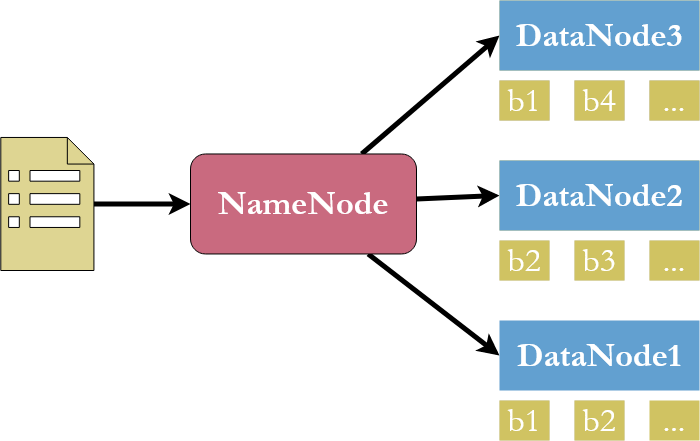
\includegraphics[width=0.7\textwidth]{img/hdfs.png}
    \caption{Architettura HDFS}
    \label{fig:hdfs_architettura}
\end{figure}
